\chapter{Simulation, reconstruction and datasets}
\section{Simulation}
Accurate Monte Carlo simulations are needed in order to make sense of the
data and search for new physics phenomena. The physics of the collisions is
simulated by the event generators MadGraph~\cite{madgraph} and PYTHIA~\cite{fs:pythia}. Then, the propagation of the particles in the detector has to be worked out.
Two different types of simulation are used by the CMS collaboration: a
GEANT4-based~\cite{fs:geant} simulation, known as the \emph{Full
Simulation}, and a detector model with simplified geometry, response
evaluation and pattern recognition to decrease the processing time per
event, the \emph{Fast Simulation}~\cite{fs:fast.simulation}. Both the
FullSim and the FastSim were employed in the generation of the background
samples for our studies.

In the FullSim, the energy depositions in the sensitive detector volumes are converted to electronic
signals using algorithms based on the observed detector behavior, including the simulation of
electronics noise and cross-talk. In many cases, the simulated electronic parameters are identical to
those of the real electronics; the constants specifying performance, calibrations, and noise behavior
can be read from the same database used for the reconstruction of the real collision data. The output of
this stage is simulated data in a format identical to that of the real raw data read from the detector.
Further processing uses this data to simulate the formation of the L1 and
HLT decisions using the same algorithms implemented online in the CMS trigger system. The simulated
raw data that is produced is processed in a manner identical to that of the real data from
LHC collisions.

The FastSim makes a number of approximations:
\begin{description}
    \item[CMS geometry:] the FastSim describes the detector with a simplified geometry of nested cilyndrical layers. The particles are propagated from one layer to the next.
    \item[Material effects:] five effects are taken into account. These are bremsstrahlung, photon conversion, multiple Coulomb scattering, energy loss through ionization and nuclear interactions. All of these are calculated analytically, except for nuclear interactions, since no analytical description is sufficient to describe the effect. Cross sections are taken from the PDG and the kinematics are derived from single particle collisions saved beforehand.
    \item[Track reconstruction:] the reconstruction is not usually part of the simulation. The FastSim includes it because, given the low fake rate in the reconstruction, it is possible to emulate it at a lower computational cost. Only the hits of the simulated track are used to make a track candidate. 
    \item[Muons:] muons are propagated through the tracker and calorimeters with average energy loss, then $dE/dx$ and multiple scattering in the iron yokes of the muon chambers are computed. Muon simulated hits are produced in all sections of the muon systems.
    \item[Calorimeters:] electron showers in the ECAL are simulated with the Grindhammer~\cite{fs:grindhammer} parametrization. Photons undergo pair conversions based on the number of radiation lengths they have traversed. Detector effects such as energy leakage into the crystal gaps and into the HCAL are included, as well as electronic noise. Shower simulation in the HCAL is similar, with different types of particles parametrized from FullSim results.
\end{description}

\section{The reconstruction of physics objects and the particle flow algorithm}
The particle flow~\cite{pf:particle.flow} (PF) event reconstruction aims at reconstructing and identifying all stable particles in the event. The essential idea is to analyse the event combining the information from all the available subdetectors in an optimal way.

The CMS detector, with its large silicon tracker and its extremely precise electromagnetic calorimeter, appears to be ideally suited for this purpose. The fundamental building bricks of the PF reconstruction are charged particle tracks, ECAL and HCAL clusters and muon tracks. These must be delivered with a high efficiency and low fake rate even in high-density environments like jets. A jet is a collection of particles resulting from the decay of a quark or gluon and emitted in the direction of the primary particle. 

Reconsider the design of the detector in figure~\ref{fig:cms_transverse}. The logic you use to
interpret this diagram is akin to that employed by the PF.
An ECAL cluster not linked to any track is a photon, an ECAL and HCAL cluster matched to a track gives a charged hadron, while an HCAL cluster without a track identifies a neutral hadron. Electrons are basically ECAL-only clusters linked to a track. Muons are by far the easiest particles to recognize.

From these basic elements, composite objects can be reconstructed, such as
$\tau$ leptons from their decay products, jets and
missing transverse energy from all the particles in the event.

Quality requirements are needed in the reconstruction of the physics
objects: thousands of particles are created in each event and their tracks
can overlap.
The quality selections are the result of detailed studies by the CMS
collaboration, aiming for the best compromise between purity and efficiency.
These recommendations are described in the following paragraphs.

\subsection{Muon reconstruction}
Muons are not stopped inside the CMS detector and leave only a tiny fraction
of their energy in the calorimeters. The information from the tracking
system and the muon chambers is exploited for their reconstruction.
The two systems are used independently in a first phase, where two
algorithms are used:
\begin{description}
    \item[The global muon reconstruction], or the \emph{outside-in}
        approach, starts from a segment in the drift tubes or cathode strip
        chambers and extrapolates the seed layer by layer up to the
        tracker. If a matching track is found in the tracking system, the
        information from both tracks is combined to improve the resolution.
    \item[The tracker muon reconstruction], or the \emph{inside-out} method,
        extrapolates a track from the inner system to the muon chambers. The
        small energy loss due to interactions with the material of the
        magnets and calorimeters is taken into account, as well as an
        uncertainty arising from the possibility of multiple scattering.
\end{description}
The recommended selection requires these two algorithms to agree, as this
improves the resolution for high-$\pt$ muons
(figure~\ref{fig:muon_resolution}).

\begin{figure}[htb]
    \centering
    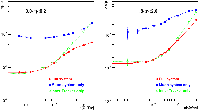
\includegraphics[width=\textwidth]{images/pdf/muon_momentum_resolution}
    \caption{Muon momentum resolution as a function of \pt in regions with
    different pseudorapidity. The blue squares are for the muon system only,
the green circles for the inner tracker only, and the red circles for the
combined reconstruction}
    \label{fig:muon_resolution}
\end{figure}

One of the most important observables for the muon candidates is the
\emph{relative isolation}. It indicates the amount of energy collected in
the vicinity of the muon, by summing the contributions from the tracking
system, the ECAL and the HCAL, divided by the \pt of the muon.
The sum runs over all deposits within a cone of radius $\Delta R = 0.3$
centred on the muon track, as illustrated in figure~\ref{fig:muon_isolation}.

\begin{figure}[htb]
    \centering
    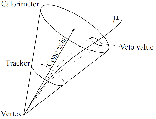
\includegraphics[width=.7\textwidth]{images/pdf/muon_isolation}
    \caption{Illustration of the isolation observable.}
    \label{fig:muon_resolution}
\end{figure}

\subsection{Electron reconstruction}

